\section{Design}
\label{sec:design}
\subsection{Design Overview}

\begin{figure*}[tb]
\centering
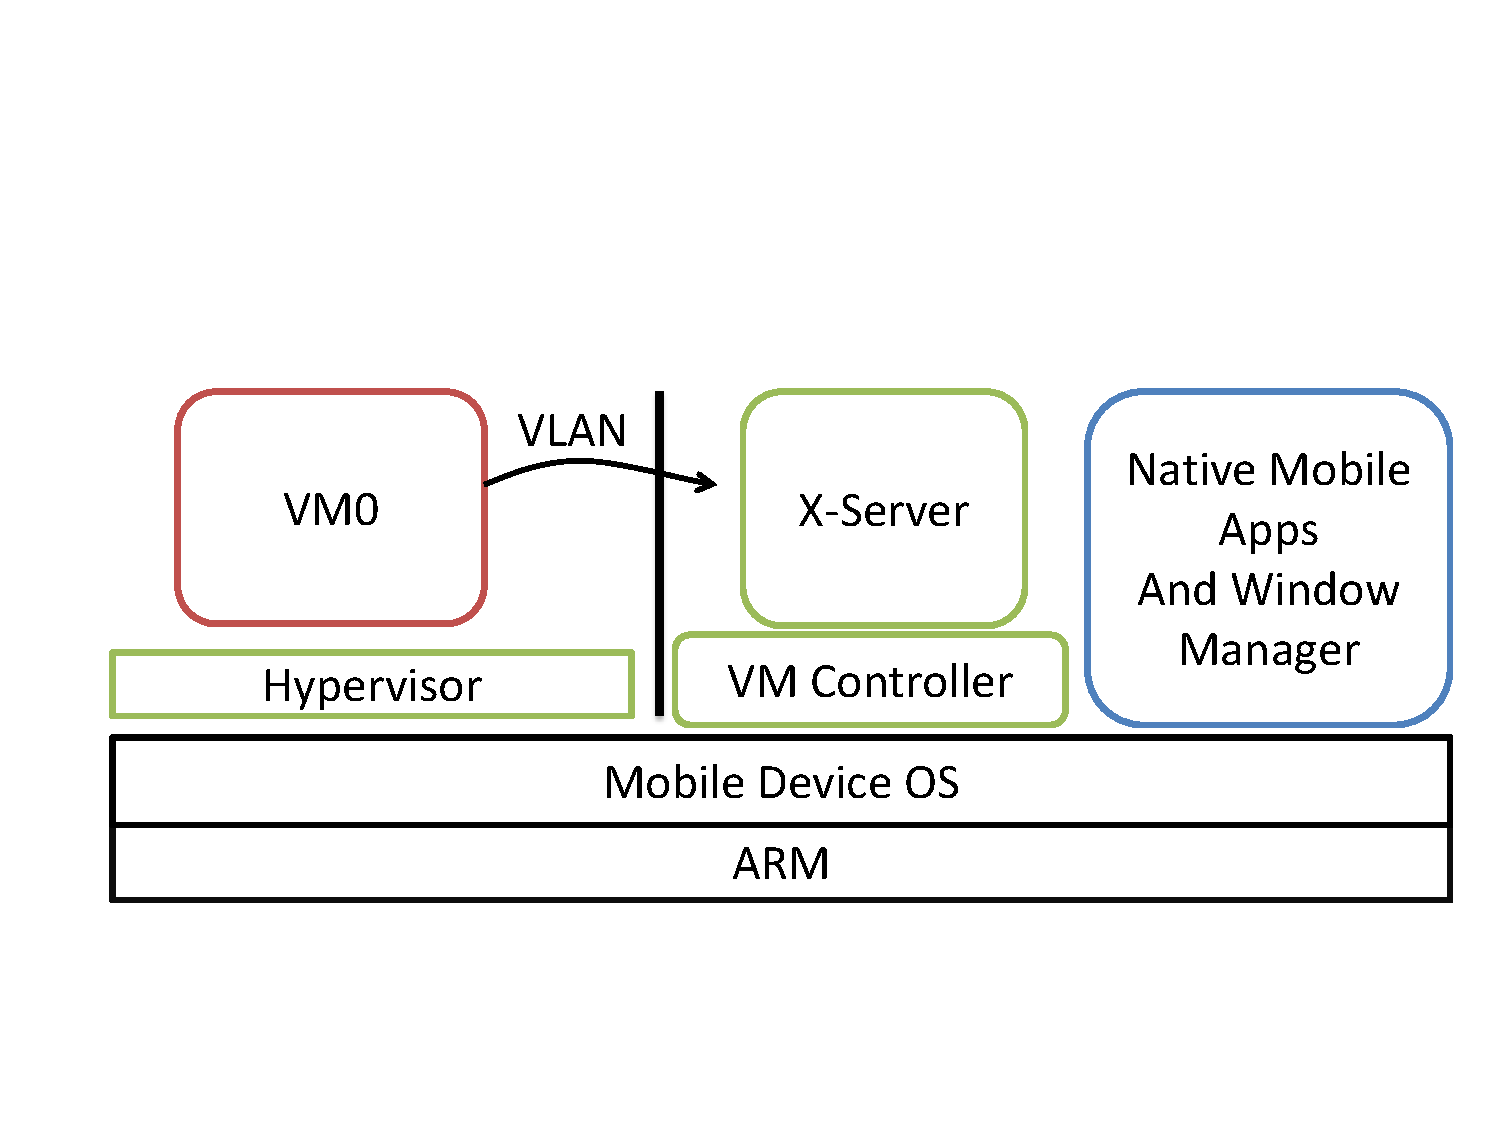
\includegraphics[width=1.5\columnwidth]{arch}
\caption{Architecture diagram}
\label{fig:arch}
\end{figure*}

\label{sec:proposedarch}
Our architecture has two main components: the virtualization framework, and the integration front-end.  The virtualization framework contains the hypervisor (KVM, UserMode Linux, or L4 based) or a container-ready kernel (Linux Containers-LXC) as well as each of the spawned VMs or containers (see Figure \ref{fig:arch}).  A VM would contain a thin OS for running the third-party application and a container could contain one or more applications.  Initially we intended to explore both x86-based Operating Systems as well as ARM based systems.  However, initial results show that x86-based Operating Systems will be far too slow.  Although an x86-based OS would have enabled a more diverse set of target applications, ARM-based systems have less virtualization overhead and some options may not be prohibitively slow. %Each of the VMs will headless themselves, but will render their applications by connecting to the native X-server. *Is this still true?* \\

The other component is the integration front-end. This contains a light X-server that has been integrated into the host OS, and also contains the VM/container controller. The controller will either run inside the X-server as a native application (ARM-based), or as a separate application within the host OS or containers. The controller will be the user interface that controls launching, switching, suspending, resuming, migrating the VMs or containers, as well as ensuring the X-server is running properly. %Most of this actual logic and functionality will be implemented by the hypervisor in the virtualization framework. \\

A shared X-server removes rendering overhead from each VM or container and reduces the complexity in composing the UI. We choose to share the rendering state between third-party applications for performance reasons and simplicity of design, but ensure isolation from native applications. Additionally the X-server runs native code, which allows for it to be less CPU intensive than running inside a VM or container. \\

We aim to make the virtualization framework device independent, which is important because we anticipate this to be the more complex component. The integration front-end will have to be ported for each new device we support, but we will strive to make its implementation simple. Our first implementation focuses on one particular device and OS and support  migration of applications from desktops. \\

In summary, we leverage an existing virtualization environment to build a secure, usable and portable framework for mobile device virtualization. Our contributions are focused on providing the ability for live migration of applications with deep integration to the mobile device. Our proposed security model is an effective method to isolate applications and we find that our design ideas are similar to other recent efforts \cite{grier2008secure} in isolating untrusted code.

\subsection{Virtualization on ARM}
The two primary goals of our design is to a. Provide isolation of selected applications on mobile phones and b. To build a usable solution which can be integrated seamlessly into the host operating system of the smartphone. To achieve the first goal, we first investigated Type-II virtualization techniques which allow a guest operating system to run from within the host operating system. The ARM architecture is not directly virtualizable as there privileged instructions which when executed by the guest operating system, do not trap to the host kernel. There are many existing techniques like dynamic binary translation, trap-and-emulate using hardware extensions, translate to trap, paravirtualization which have been used in existing virtualization solutions for x86. QEMU \cite{qemu} is one of the more recent, popular and opensource virtual machine monitors that can be used to run operating systems built for different architectures to run on different machines. QEMU relies on dynamic binary translation and has been ported to run on multiple platforms like ARM, PowerPC, i386 etc. Our first implementation uses QEMU and attempts to address the initial design goal of evaluating the overhead of dynamic binary translation on a smartphone running an ARM processor. Results from our preliminary investigations are presented in \ref{sec:eval} and we plan to investigate other techniques listed below.

\subsection{Other Virtualization Techniques}
The following list presents the different techniques that we are considering to have a faster, more usable and secure solution.
\subsubsection{KVM}
The Kernel Virtual Machine Monitor (KVM) is a virtualization technique in which the Linux kernel plays the role of a hypervisor. In traditional virtualization tools like Xen \cite{xen}, a hypervisor manages the scheduling, memory management and driver support for the different guest operating systems. Since the linux kernel already performs most of these tasks for the host operating system, it is efficient to re-use this functionality for the guest operating systems too. KVM consists of a kernel module, which introduces a guest mode,  page tables and handles privileged instructions through a `trap-and-emulate' scheme. On the x86 architecture KVM uses hardware virtualization extensions like the Intel VT or AMD-V for the same. 
The ARM architecture is not strictly virtualizable as there are privileged instructions which do not trap to the kernel and therefore a simple `trap-and-emulate' approach cannot be used. Hence more complex techniques like dynamic binary translation, translation to add software interrupts or paravirtualization are required for porting KVM to ARM. There have been some initial attempts to port KVM to ARM \cite{columbia} but the high performance overhead reported leads us to explore other solutions for isolation and security. 

\subsubsection{User Mode Linux}
User Mode Linux (UML) is a virtualization technique in which the guest operating systems run as user mode processes inside the host. When compared to hypervisors like VMWare ESX or Xen, UML offers a simpler solution and is patched into the Linux kernel source tree. The first version of User Mode Linux used \emph{ptrace} to virtualize system calls and modify and divert them into the user space kernel for execution. Later versions of UML introduced the Separate Kernel Address Space (SKAS) mode  where the UML kernel runs in a different address space from its processes. This addresses security issues by making the UML kernel inaccessible to the UML processes and also provides a noticeable speedup. Also this technique is only effective when the architecture of the guest operating system is the same as the host and fits the design constraints of our problem. User Mode Linux was built originally on the i386 architecture and has since been extended to the PowerPC and x86\_64 architectures. Technically it should be feasible to port UML to ARM architecture. \\
Some downsides of using UML are that the amount of overhead is relatively large for workloads which have a number of interrupts and the project is not under active development anymore. We plan to explore porting UML to ARM and measure the overhead caused in the weeks ahead. 

\subsubsection{Linux Containers}
Linux Containers (LXC) implement OS-level virtualization techniques in order to run a number of isolated virtual environments on a single host.  LXC differs from conventional virtualization techniques, which generally require the installation of guest OSes.  The isolated virtual environments or containers, are built upon other Linux security mechanisms.  Resource namespaces allow containers to manipulate the accessing of processes, files, and hardware resources.  Control groups are used to limit the resources used by a container.  Capability bounding sets reduce a container's privileges.  

Unlike with conventional virtualization, LXC has almost no overhead as it does not require guest OSes or dynamic binary translation.  On the other hand, because it is a OS-level virtualization technique and runs processes on a Linux kernel, other OSes such as Windows and other UNIXes (BSD or OSX) can not be used as containers.  

The main obstacle to using Linux Containers are the requirements.  LXC requires a Linux kernel version 2.6.27 or greater, and the Pre is running 2.6.24.  The kernel functionality would have to be back ported in order to work with the Pre.  The Android is running 2.6.29; however, porting the LXC tools to Android will likely be very difficult.
